\documentclass{sigchi}

% Use this command to override the default ACM copyright statement (e.g. for preprints). 
% Consult the conference website for the camera-ready copyright statement.


%% EXAMPLE BEGIN -- HOW TO OVERRIDE THE DEFAULT COPYRIGHT STRIP -- (July 22, 2013 - Paul Baumann)
% \toappear{Permission to make digital or hard copies of all or part of this work for personal or classroom use is 	granted without fee provided that copies are not made or distributed for profit or commercial advantage and that copies bear this notice and the full citation on the first page. Copyrights for components of this work owned by others than ACM must be honored. Abstracting with credit is permitted. To copy otherwise, or republish, to post on servers or to redistribute to lists, requires prior specific permission and/or a fee. Request permissions from permissions@acm.org. \\
% {\emph{CHI'14}}, April 26--May 1, 2014, Toronto, Canada. \\
% Copyright \copyright~2014 ACM ISBN/14/04...\$15.00. \\
% DOI string from ACM form confirmation}
%% EXAMPLE END -- HOW TO OVERRIDE THE DEFAULT COPYRIGHT STRIP -- (July 22, 2013 - Paul Baumann)


% Arabic page numbers for submission. 
% Remove this line to eliminate page numbers for the camera ready copy
\pagenumbering{arabic}


% Load basic packages
\usepackage{balance} % to better equalize the last page
\usepackage{graphics} % for EPS, load graphicx instead
\usepackage{times}  % comment if you want LaTeX's default font
\usepackage{url}   % llt: nicely formatted URLs
\usepackage{listings}
\usepackage{color}
\usepackage[english]{babel}
\usepackage{setspace}

\definecolor{mygreen}{rgb}{0,0.6,0}
\definecolor{mygray}{rgb}{0.5,0.5,0.5}
\definecolor{mymauve}{rgb}{0.58,0,0.82}
\definecolor{black}{rgb}{0,0,0}

\lstset{ %
  backgroundcolor=\color{white},   % choose the background color; you must add \usepackage{color} or \usepackage{xcolor}
  basicstyle=\scriptsize\ttfamily,        % the size of the fonts that are used for the code
  breakatwhitespace=false,         % sets if automatic breaks should only happen at whitespace
  breaklines=true,                 % sets automatic line breaking
  captionpos=b,                    % sets the caption-position to bottom
  commentstyle=\color{mygreen},    % comment style
  deletekeywords={...},            % if you want to delete keywords from the given language
  escapeinside={\%*}{*)},          % if you want to add LaTeX within your code
  extendedchars=true,              % lets you use non-ASCII characters; for 8-bits encodings only, does not work with UTF-8
  frame=single,                    % adds a frame around the code
  keepspaces=true,                 % keeps spaces in text, useful for keeping indentation of code (possibly needs columns=flexible)
  keywordstyle=\color{blue},       % keyword style
  %language=Octave,                 % the language of the code
  morekeywords={*,...},            % if you want to add more keywords to the set
  numbers=left,                    % where to put the line-numbers; possible values are (none, left, right)
  numbersep=5pt,                   % how far the line-numbers are from the code
  numberstyle=\tiny\color{mygray}, % the style that is used for the line-numbers
  rulecolor=\color{black},         % if not set, the frame-color may be changed on line-breaks within not-black text (e.g. comments (green here))
  showspaces=false,                % show spaces everywhere adding particular underscores; it overrides 'showstringspaces'
  showstringspaces=false,          % underline spaces within strings only
  showtabs=false,                  % show tabs within strings adding particular underscores
  stepnumber=2,                    % the step between two line-numbers. If it's 1, each line will be numbered
  stringstyle=\color{black},     % string literal style
  tabsize=2,                       % sets default tabsize to 2 spaces
  title=\lstname                   % show the filename of files included with \lstinputlisting; also try caption instead of title
}

% llt: Define a global style for URLs, rather that the default one
\makeatletter
\def\url@leostyle{%
 \@ifundefined{selectfont}{\def\UrlFont{\sf}}{\def\UrlFont{\small\bf\ttfamily}}}
\makeatother
\urlstyle{leo}


% To make various LaTeX processors do the right thing with page size.
\def\pprw{8.5in}
\def\pprh{11in}
\special{papersize=\pprw,\pprh}
\setlength{\paperwidth}{\pprw}
\setlength{\paperheight}{\pprh}
\setlength{\pdfpagewidth}{\pprw}
\setlength{\pdfpageheight}{\pprh}

% Make sure hyperref comes last of your loaded packages, 
% to give it a fighting chance of not being over-written, 
% since its job is to redefine many LaTeX commands.
\usepackage[pdftex]{hyperref}
\hypersetup{
pdftitle={SIGCHI Conference Proceedings Format},
pdfauthor={LaTeX},
pdfkeywords={SIGCHI, proceedings, archival format},
bookmarksnumbered,
pdfstartview={FitH},
colorlinks,
citecolor=black,
filecolor=black,
linkcolor=black,
urlcolor=black,
breaklinks=true,
}

% create a shortcut to typeset table headings
\newcommand\tabhead[1]{\small\textbf{#1}}


% End of preamble. Here it comes the document.
\begin{document}

\title{DressCode: The Design of Computational Design Tool Through Information Ecology}

\numberofauthors{3}
\author{
 \alignauthor 1st Author Name\\
  \affaddr{Affiliation}\\
  \affaddr{Address}\\
  \email{e-mail address}\\
  \affaddr{Optional phone number}
 \alignauthor 2nd Author Name\\
  \affaddr{Affiliation}\\
  \affaddr{Address}\\
  \email{e-mail address}\\
  \affaddr{Optional phone number}
}

\maketitle

\begin{abstract}
\end{abstract}

\keywords{
	Guides; instructions; author's kit; conference publications;
	keywords should be separated by a semi-colon.
}

\category{H.5.m.}{Information Interfaces and Presentation (e.g. HCI)}{Miscellaneous}

\section{Introduction}
\section{Background}
\section{Related Work}

\section{Dress Code Software Description}
DressCode is a 2D computational design tool that is distinguished by its support of \emph{linked editable representations} of a design in two forms: programmatic and graphic. As designs create and manipulate forms graphically, the software generates readable, editable programming expressions that correspond to their actions. designs can also generate graphic forms by writing programming expressions and manipulate these forms with the graphic editing tools. Here, we describe the interface and toolset of DressCode, the interaction paradigm by which a design creates a design, and the technical implementation that facilitates this paradigm.

\begin{figure*}
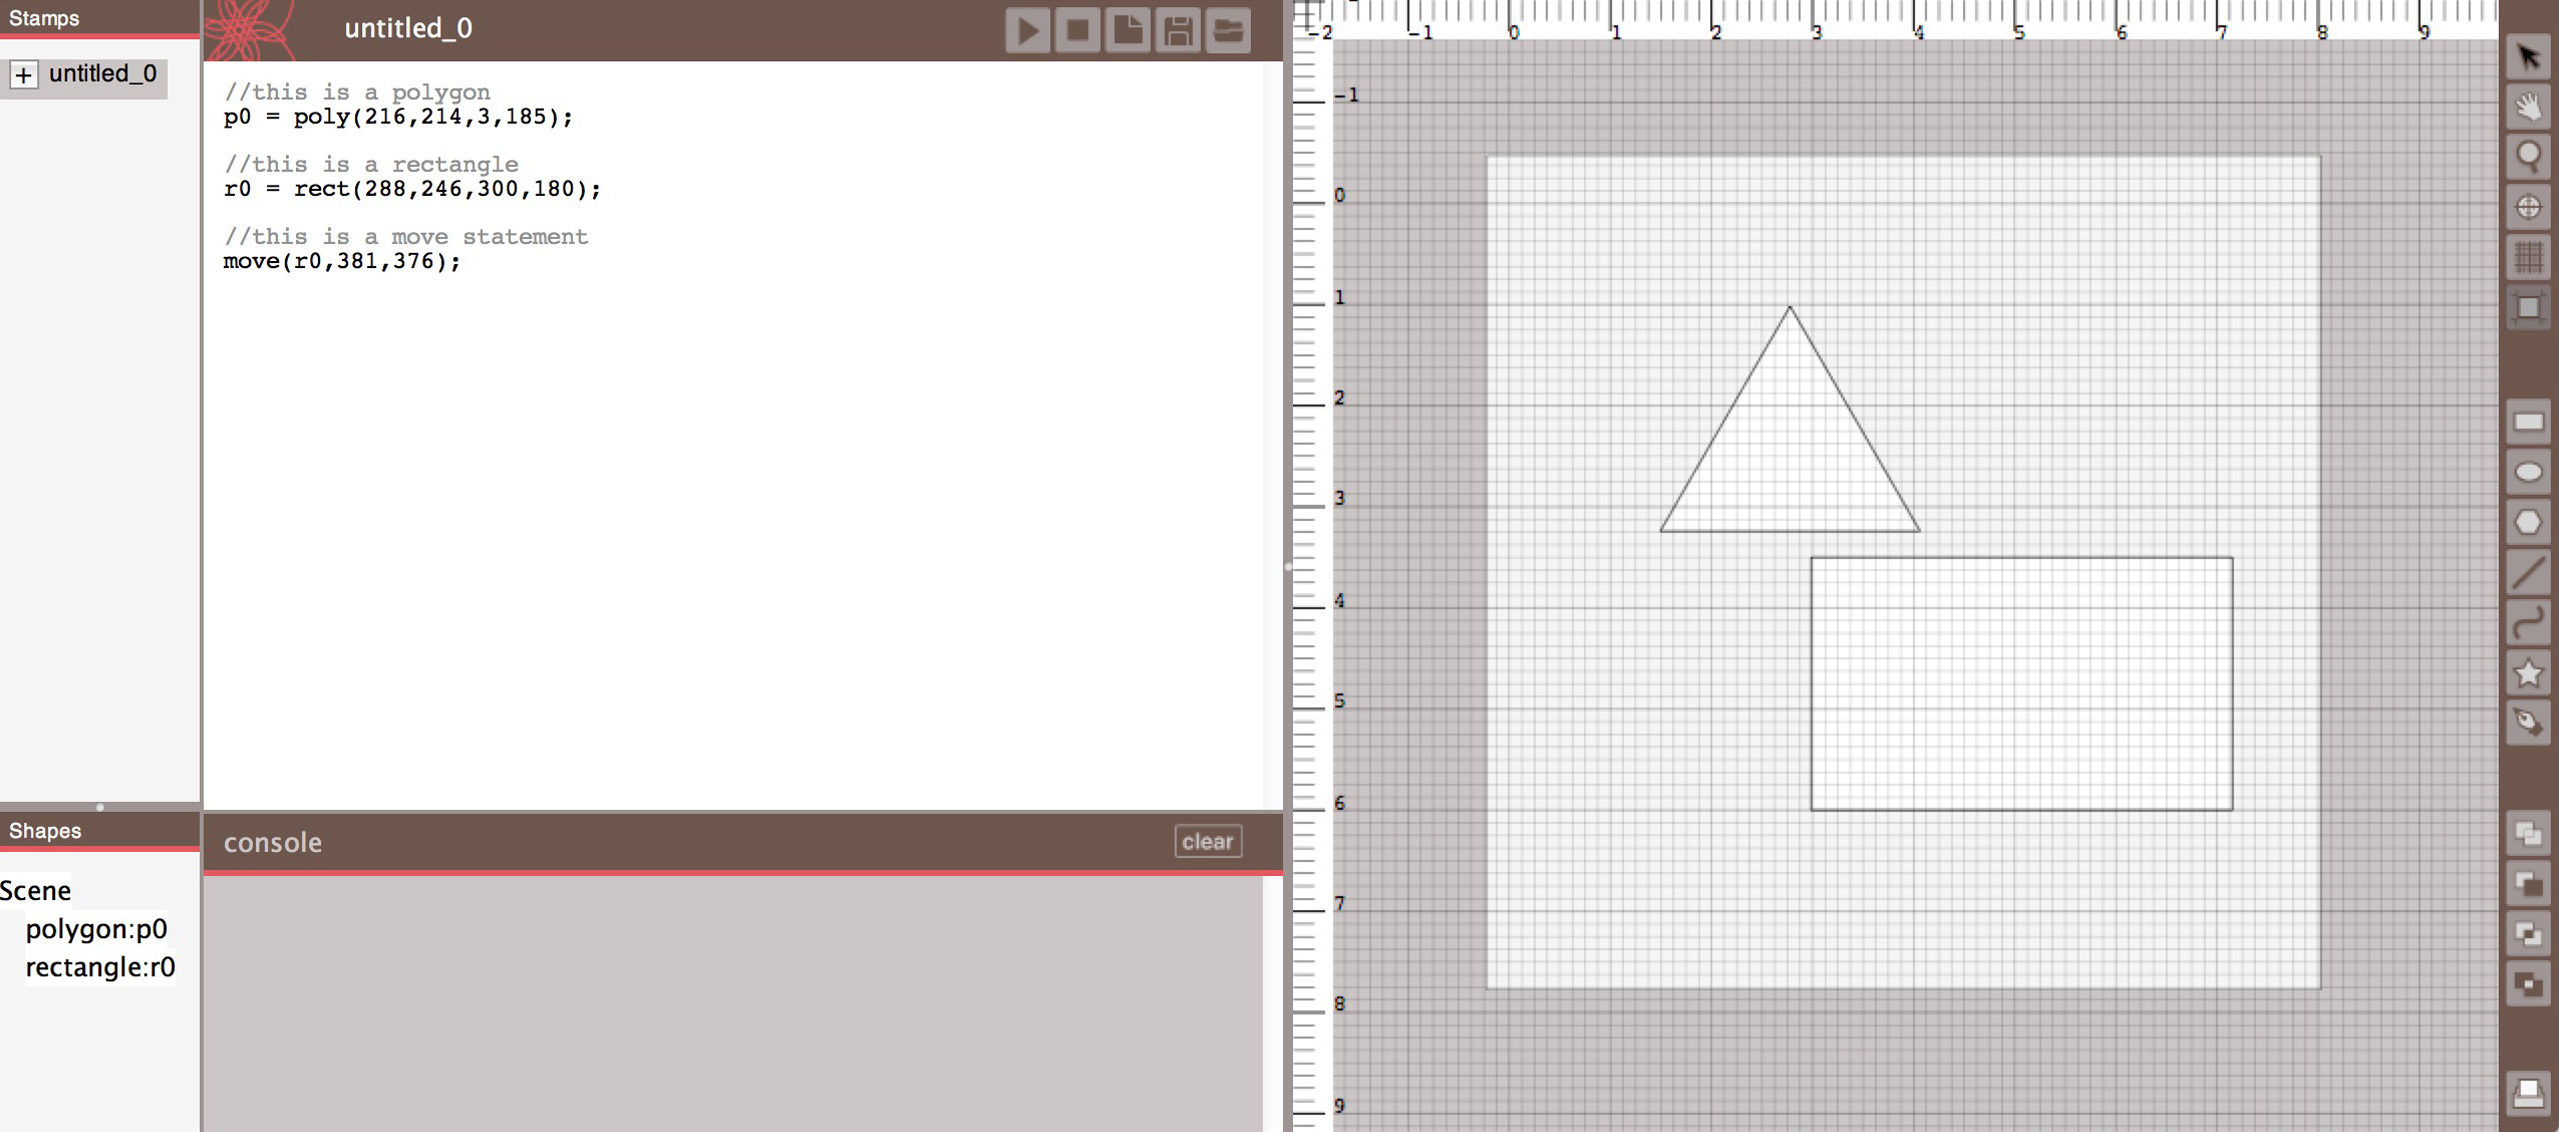
\includegraphics[width=\textwidth]{images/application_image_sm_content.jpg}
\caption{The DressCode Software)}
\label{fig:application_image}
\end{figure*}

\subsection{System Overiew}
The DressCode application resmbles a mashup of a digital graphic drawing tool, and a text editor. The interface iself it divided into two primary panels; a graphic panel on the right and a text editor panel on the left (figure:\ref{fig:application_image}). A design may write and execute programs using the text editor; similarly they can draw and manipulate shapes using the mouse in the graphic panel. Each panel contains specific features and tools to enable these respective interactions. The text editor contains a console for output and error messages, and a panel with buttons for compiling and running the current program, and terminating the compilation process. The design panel contains a re-sizable drawing board and grid with rulers corresponding to real-world units (inches and millimeters), and pan and zoom tools to facilitate navigation. A toolbar on the right-hand side of the graphic panel contains a menu of drawing and manipulation tools. It also contains a print tool which allows the design to export their current visual design in vector format for output through printing, or 2-axis forms of digital fabrication (figure:\ref{fig:graphic_tools}).

\begin{center}
\begin{figure}[h!]

\includegraphics[width=\columnwidth]{images/graphic_tools.jpg}
\caption{The graphic drawing and manipulation tools in DressCode (from left to right: selection and move tool, rectangle tool, ellipse tool, regular polygon tool, line tool, curve tool, SVG import tool, pen tool)}
\label{fig:graphic_tools}
\end{figure}
\end{center}
\vspace{-20pt}

The graphic drawing tools include regular primitive creation tools and a pen tool for the creation of irregular forms.  In addition to the drawing tools, the selection tool allows for individual primitives and groups to be manually selected and moved, and the boolean operation tools allow for the combination of two or more forms into a unified shape through a variety of polygon boolean operators (union, difference, intersection and either/or). The interface also contains two additional panels, the stamp panel and the declarative view which are described in the organizational structures subsection.

 DressCode contains a custom functional programing language which enables 2D drawing functionality via text expressions. The language supports conventional programming data-types, as well as loops, conditional expressions and design-defined functions. Variables in DressCode are dynamically typed and identifiers can be assigned to data-types that differ from their original assignment. The DressCode language contains a subset of expressions which facilitate the drawing and transformation of 2D graphic geometric forms. Lastly, the language supports basic math expressions and enables a variety of random noise generation methods. We discuss the drawing elements of the DressCode programing language and their relationship with the graphic manipulation tools at length in the following section. A note on terminology: for the remainder of this paper, we denote actions made in the graphic panel with the mouse as \textit{graphic actions}, and actions made in the programing panel by typing expressions as \textit{programatic actions}.


\subsection{Linked Representations In Practice}
Graphic tools and programing tools each have their own design affordances. Graphic tools are based on the metaphor of drawing and manipulation with traditional media, and often represented by icons and symbols reflecting this metaphor. As a result, they can be intuitive or inviting to new designs. Textual programing tools are often less intuitive, but have the advantage of readily supporting complexity and automation in design, and are a natural fit for parametric representations. Because of their differences, combining computational and graphic design into a unified interaction raises many questions and opportunities for different forms of interaction: What forms of interaction best support the distinct affordances of graphic manipulation and programing? How should graphical organizational structures be reconciled with computational forms of organization? What rules dictate the resolution of inevitable conflicts between graphical and programmatic actions? How does the intended application of the software dictate the relationships between the two paradigms?

In respect to these questions, we describe the DressCode's interaction structure, which we have based on primary design principles: Symmetry and Readability. In this section, we describe the latest state of the tool, which was iteratively developed through a series of workshops. The workshops not only directed the iterations of the tool itself, but assisted in the clarification of the design principles behind it. We discuss this development process at length in the workshop section. For now, we will describe the specific structures of the current version of DressCode as they correspond to symmetry and readability.

\subsection{Symmetry}
The governing design principle in DressCode is symmetry between programmatic actions and graphic actions. For every drawing-oriented programmatic action in a designs' program, a graphic element is generated or manipulated in the graphic view. Conversely, for each graphic action, a corresponding programing expression (or set of expressions) will appear in the text editor, within the lines of the designer's program. The DressCode programing language syntax was developed expressly to support this translation. 

\subsubsection{Auto-generated programing expressions}
The drawing API is formulated on an Object Oriented Programming paradigm where basic shapes (points, lines, curves, polygons etc.) are initialized by calling the appropriate method and passing it a set of parameters designating it's location and dimensions. If a shape is generated graphically, it's parameters are determined by the mouse gestures of the designer (where they click to determine the origin, and how far they drag from the origin to determine the dimensions). A new programing expression appears in the designer's program with its method determined by the type of graphic tool that was used to create the shape, and the parameters determined by the graphically defined dimensions. (points, lines, curves, polygons etc.) Shapes are layered in a design in order of the designer's graphic and programmatic actions, with shapes that were drawn most recently appearing on top of those created earlier.

Transformation methods, including moving, scaling, rotation, color and stroke changes, and shape booleans follow a similar structure to shape initialization. In the DressCode programing language, transformations are performed by either wrapping a shape-initialization expression in an a transformation expression, or by assigning an identifier to the shape, and then calling the transformation method with the identifier. Each graphic transformation tool corresponds to a transformation method in the DressCode language and every transformation graphic action generates a programing expression in the programing panel which contains as its first argument a reference to the shape which was selected and manipulated graphically. Throughout the design process, a complete representation of the current state of the graphic design is continually maintained in the programming panel. This representation allows programs to be shared and remixed easily; if the textual program from one design is copied and inserted into another designs' program, it will re-generate the exact design in the context of the new  design. 

\subsubsection{Static and Dynamic Generativity}
DressCode contains functionality to help people organize their code in the form of static and dynamic \textit{stamps}: graphically created functions that return shape primitives. Dynamic stamps are created by selecting a portion of code in a user's program and then selecting the dynamic stamp option from the menu. A dynamic stamp will package the selected code in a function with a name specified by the user. Static stamps are created by graphically selecting a single primitive or group with either the selection tool or the declarative view, and selecting the static stamp option. Static stamps translate shapes generated in random positions to explicit primitives, allowing users to save a specific instances of a generative design (see Figure \ref{fig:stamps}).
Stamps are listed in the stamp menu and can be added to a user's primary program by selecting the \textit{+} icon next to each stamp. The code of both static and dynamic stamps can be modified by the user as the code generated is human readable.

\begin{center}
\begin{figure}[h!]
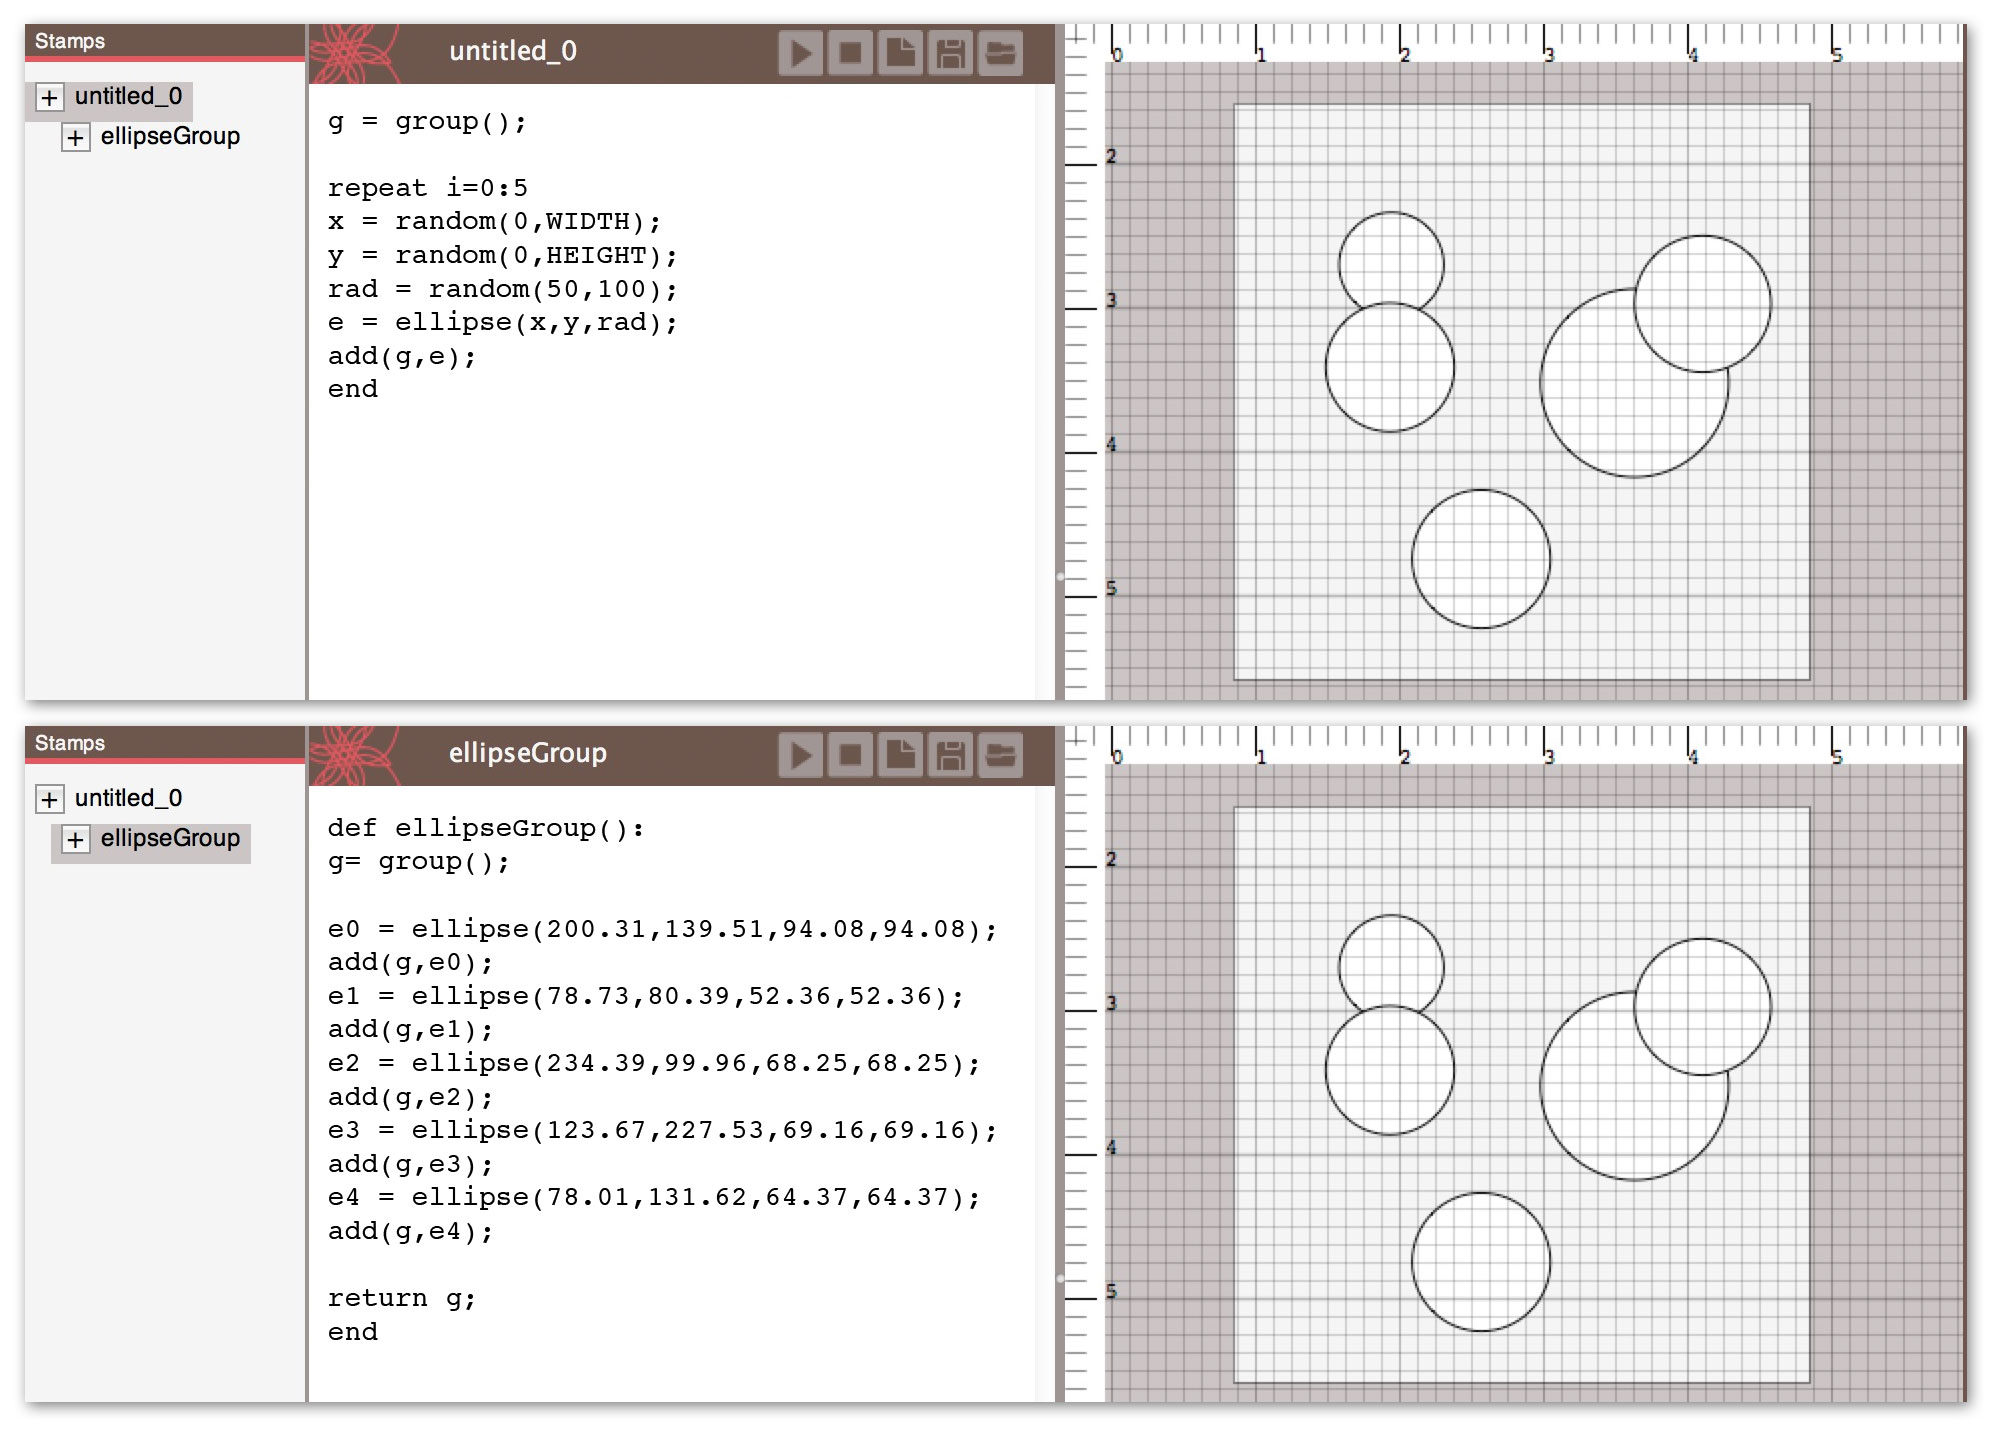
\includegraphics[width=\columnwidth]{images/stamps.jpg}
\caption{Static stamp functionality. (Top: User defined code which generates five random ellipses. The ellipses' positioning and size will change each time the program is run. Bottom: static stamp created from ellipses which will always return the same design.)}
\label{fig:stamps}
\end{figure}
\end{center}
\vspace{-20pt}

\subsection{Readability}
As we discovered through our implementation, Symmetry between graphic manipulation and textual programing must be tempered by concerns of usability. Merely producing a textual expression that accurately reflects a graphic action does not ensure that the interaction will be interpretable to the designer, let alone useful to their design process. We therefore attempted to make the editable linkages between programmatic and graphic actions to our target designs: novice programmers. 

\subsubsection{Expression Insertion}
First, we considered \textit{where} generated expressions appear within a program. For graphic action that initialize a new shape, the programming expression will always appear below the last line in the program. If the designer performs a transformation graphic action however, the expression will be inserted into the line below the last transformation expression of the selected shape, thereby automatically grouping shape initialization expressions with their corresponding transformations. Some of the transformation methods, including shape booleans and grouping methods result in the initialization of new shapes by combining several existing shapes. Any transformation expressions for these new shapes will subsequently appear following their initialization expression.  This results in the creation of a logically organized program through graphic edits.Naturally, in the process of manually writing code, the designer may consciously or unconsciously write expressions in a manner that deviates from this organization. Fortunately, manual edits by the designer will not prevent the auto generation method from functioning for successive graphic actions. More importantly, the consistent, simple rule-set for auto-insertion enables the designer to anticipate where expressions will be inserted into their code, which is essential as a program grows in length and complexity.

\subsubsection{Reference}
We also considered \textit{how} shapes should be referenced when transitioning between graphics and code. Similar to many functional programing languages, the DressCode language enables methods to be nested within one-another. Furthermore, there is no \textit{draw} method. Shapes that are initialized automatically appear in a design. Therefore there is a degree of flexibility and ambiguity for how a designer may employs identifiers in their code. In order to deal with this ambiguity when translating graphic actions to programmatic representations, we considered what would make a program most readable for a design. All graphic actions that create new shapes produce programmatic expressions that are automatically assigned an identifier. Subsequent transformation graphic actions will produce programmatic expressions that reference auto generated identifier on the following line. This produces code that while requiring more lines, is readable. In the case that the design problematically initializes a shape without an identifier and then transforms it graphically, the software will recognize the distinction and resort to wrapping the initialization expression in the appropriate transformation expression. if the design re-assigns or modifies the identifier of a shape through a programmatic action, future graphic actions on the shape will recognize this modification and use the new identifier.     

\subsubsection{Declarative History}
It was important to us that the \textit{history} of a design was also readable. Because the DressCode programing language employs a declarative paradigm, designs are represented as a series of the designs' actions, rather than a single state which is updated as changes are made. Therefore while a single shape in a design always has a current position, scale and rotation that determines how it is drawn at that point, the program of the design 


Declarative highlighting


why multiple expressions
History is also maintained
automatically generated identifiers
When a primitive is moved for the first time, a textual move expression is inserted into the design's program. For all subsequent moves of that primitive with the move tool, the inserted move expression is updated to reflect the new coordinates of the primitive (see Figure \ref{fig:auto_generated_code}).
%\subsubsection{Simplicity}

%Primitives can be modified through two kinds transformation methods, geometric and stylistic. Geometric transformations allow for primitives to be rotated, scaled, moved or combined with other primitives through polygon boolean operations, (union, intersection, either-or and difference), and are performed relative to the origin of the primitive, unless otherwise specified. Stylistic transformations modify the appearance of a primitive (color and stroke weight).  By using the transformation methods to manipulate primitives it is possible to generate complex and generative designs from the repetition and structured distribution of simple forms. As a method of organizing sets of primitives, DressCode contains a group datatype, a specialized list for organizing and performing collective transformations on multiple primitives. Groups facilitate more advanced transformations including clipping masks and collective merge operations. When a primitive is moved for the first time, a textual move expression is inserted into the design's program. For all subsequent moves of that primitive with the move tool, the inserted move expression is updated to reflect the new coordinates of the primitive (see Figure \ref{fig:auto_generated_code}).

 

\subsection{Technical Implementation}
Resolving conflicts between identifiers
placing elements in loops and expressions
handling functions

%\begin{center}
%\begin{figure}[h!]
%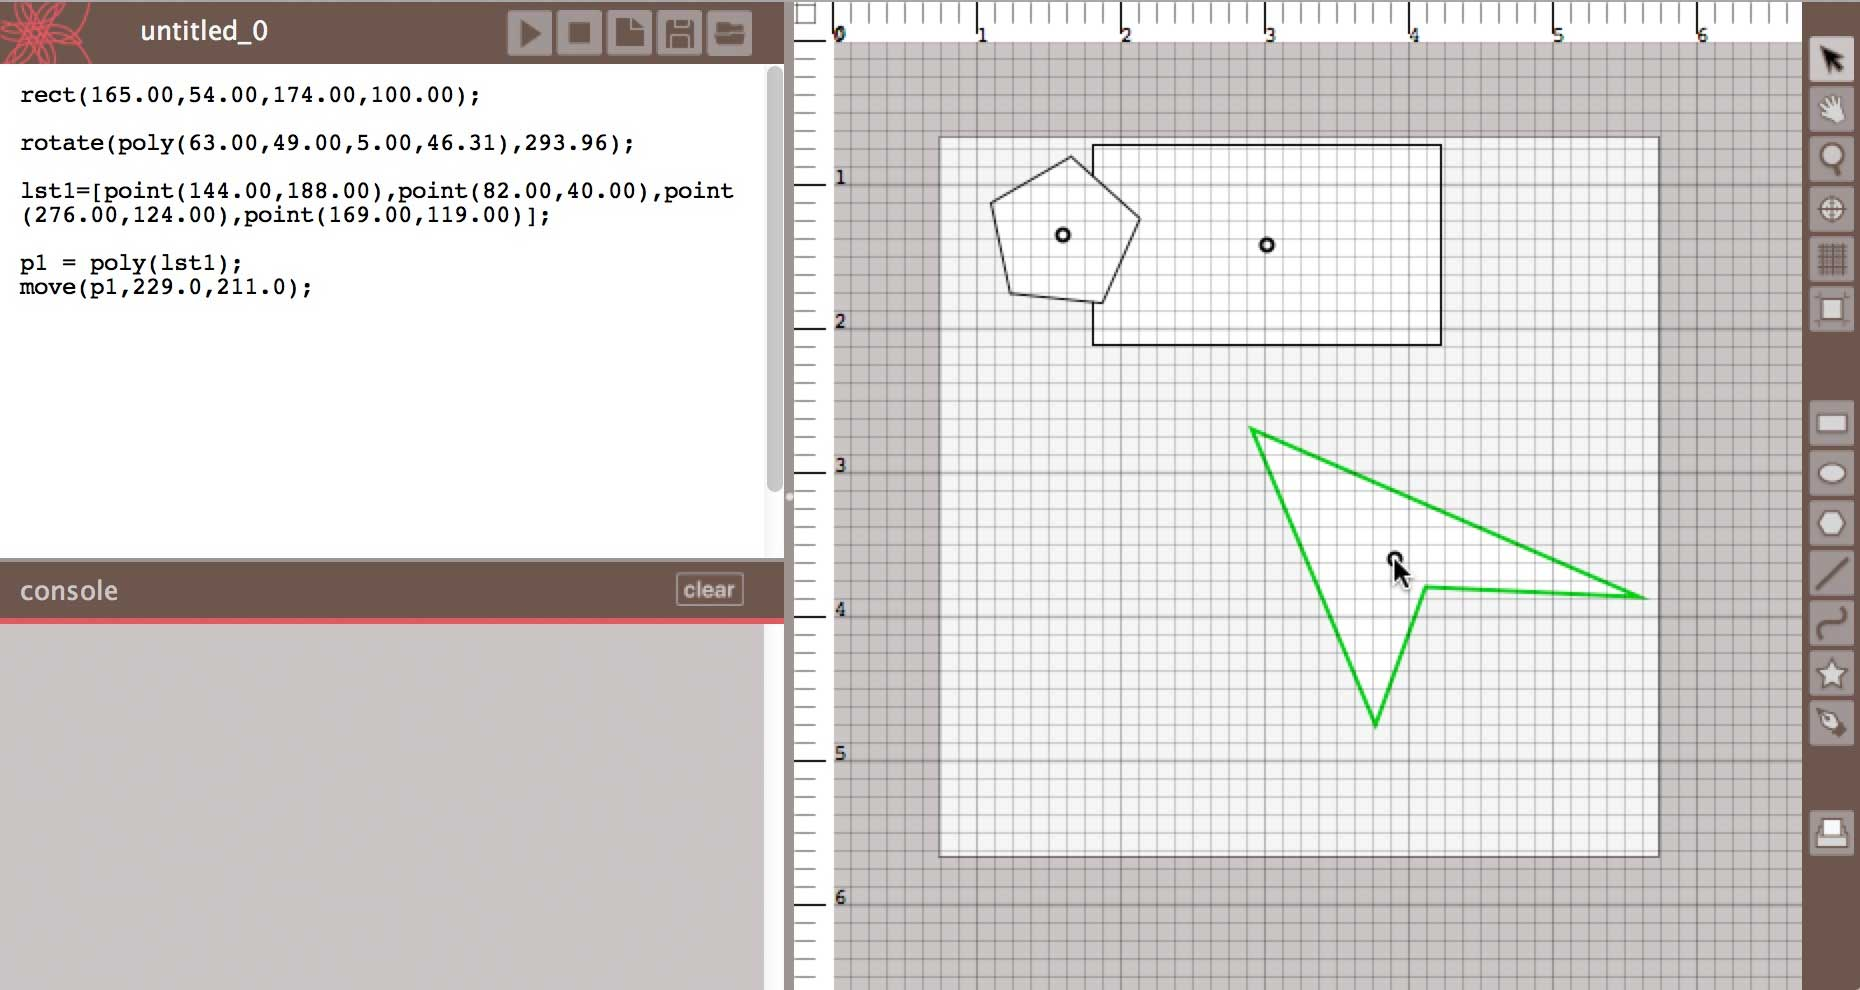
\includegraphics[width=\columnwidth]{images/auto_generated_code.jpg}
%\caption{Graphically created polygon, rectangle, and irregular polygon, and corresponding automatically-generated code. (The irregular polygon has just been moved with the selection tool.)}
%\label{fig:auto_generated_code}
%\end{figure}
%\end{center}
%\vspace{-20pt}

The declarative view contains a listing of all primitives in the current design. Child primitives are nested within their parent groups. When selected in the declarative view, the primitive is selected and highlighted in the design view, and the line where the primitive was last modified in the text-editor is highlighted (see Figure \ref{fig:declarative_view}). The declarative view is designed to provide visual feedback on how elements of a design connect to the design's program, and provide a practical selection technique for complex designs.

\begin{center}
\begin{figure}[h!]
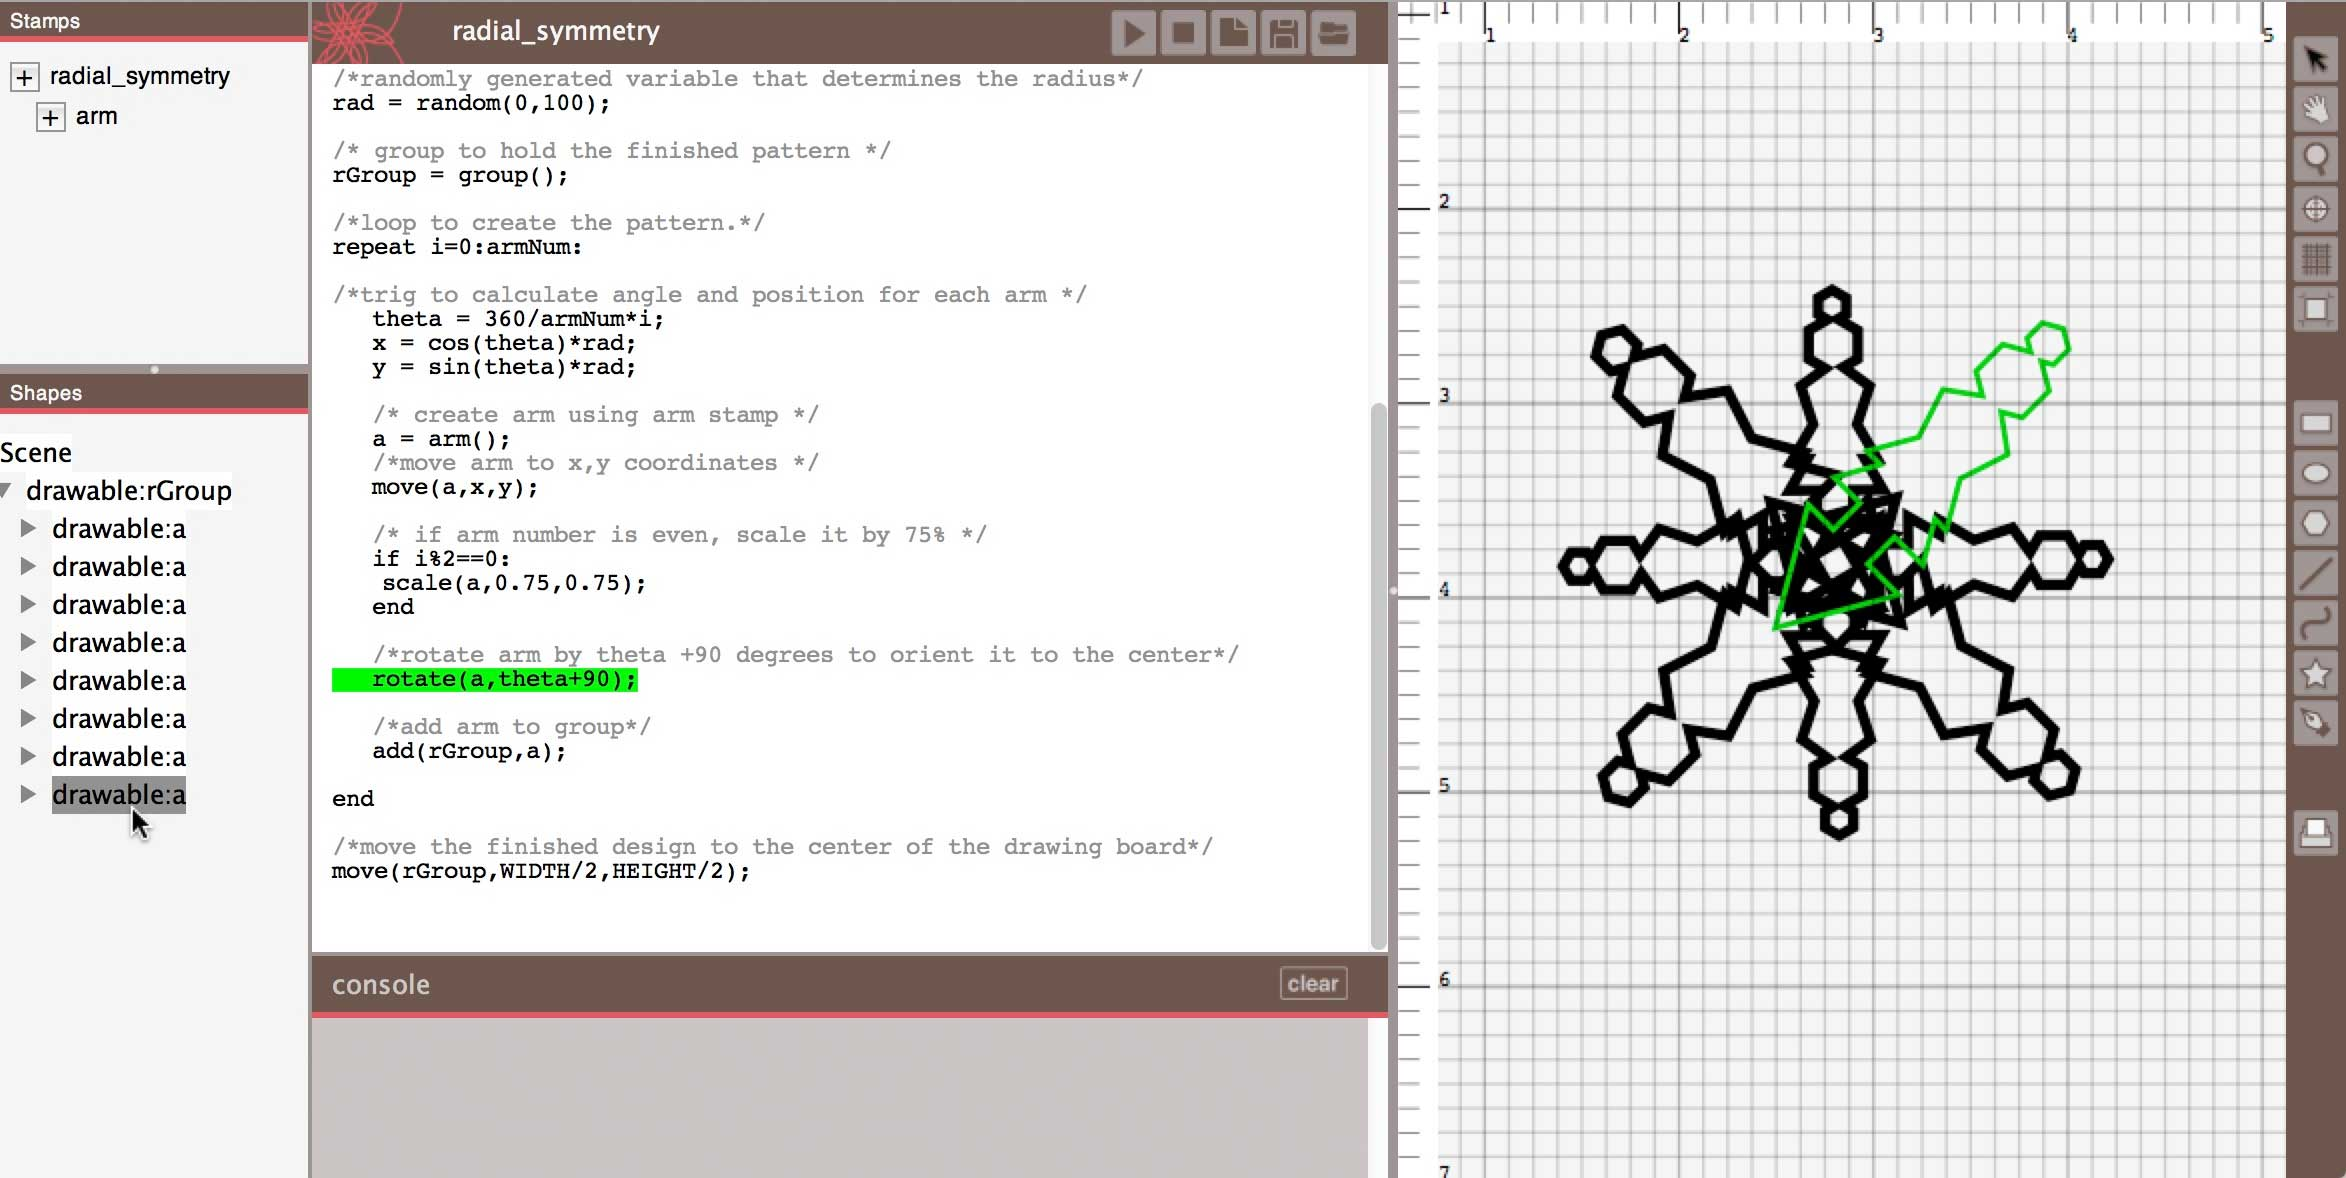
\includegraphics[width=\columnwidth]{images/selection_mechanism.jpg}
\caption{Declarative view with selected primitive}
\label{fig:declarative_view}
\end{figure}
\end{center}
\vspace{-20pt}

DressCode contains functionality to help people organize their code in the form of static and dynamic \textit{stamps}: graphically created functions that return shape primitives. Dynamic stamps are created by selecting a portion of code in a design's program and then selecting the dynamic stamp option from the menu. A dynamic stamp will package the selected code in a function with a name specified by the design. Static stamps are created by graphically selecting a single primitive or group with either the selection tool or the declarative view, and selecting the static stamp option. Static stamps translate shapes generated in random positions to explicit primitives, allowing designs to save a specific instances of a generative design (see Figure \ref{fig:stamps}).
Stamps are listed in the stamp menu and can be added to a design's primary program by selecting the \textit{+} icon next to each stamp. The code of both static and dynamic stamps can be modified by the design as the code generated is human readable.

\begin{center}
\begin{figure}[h!]
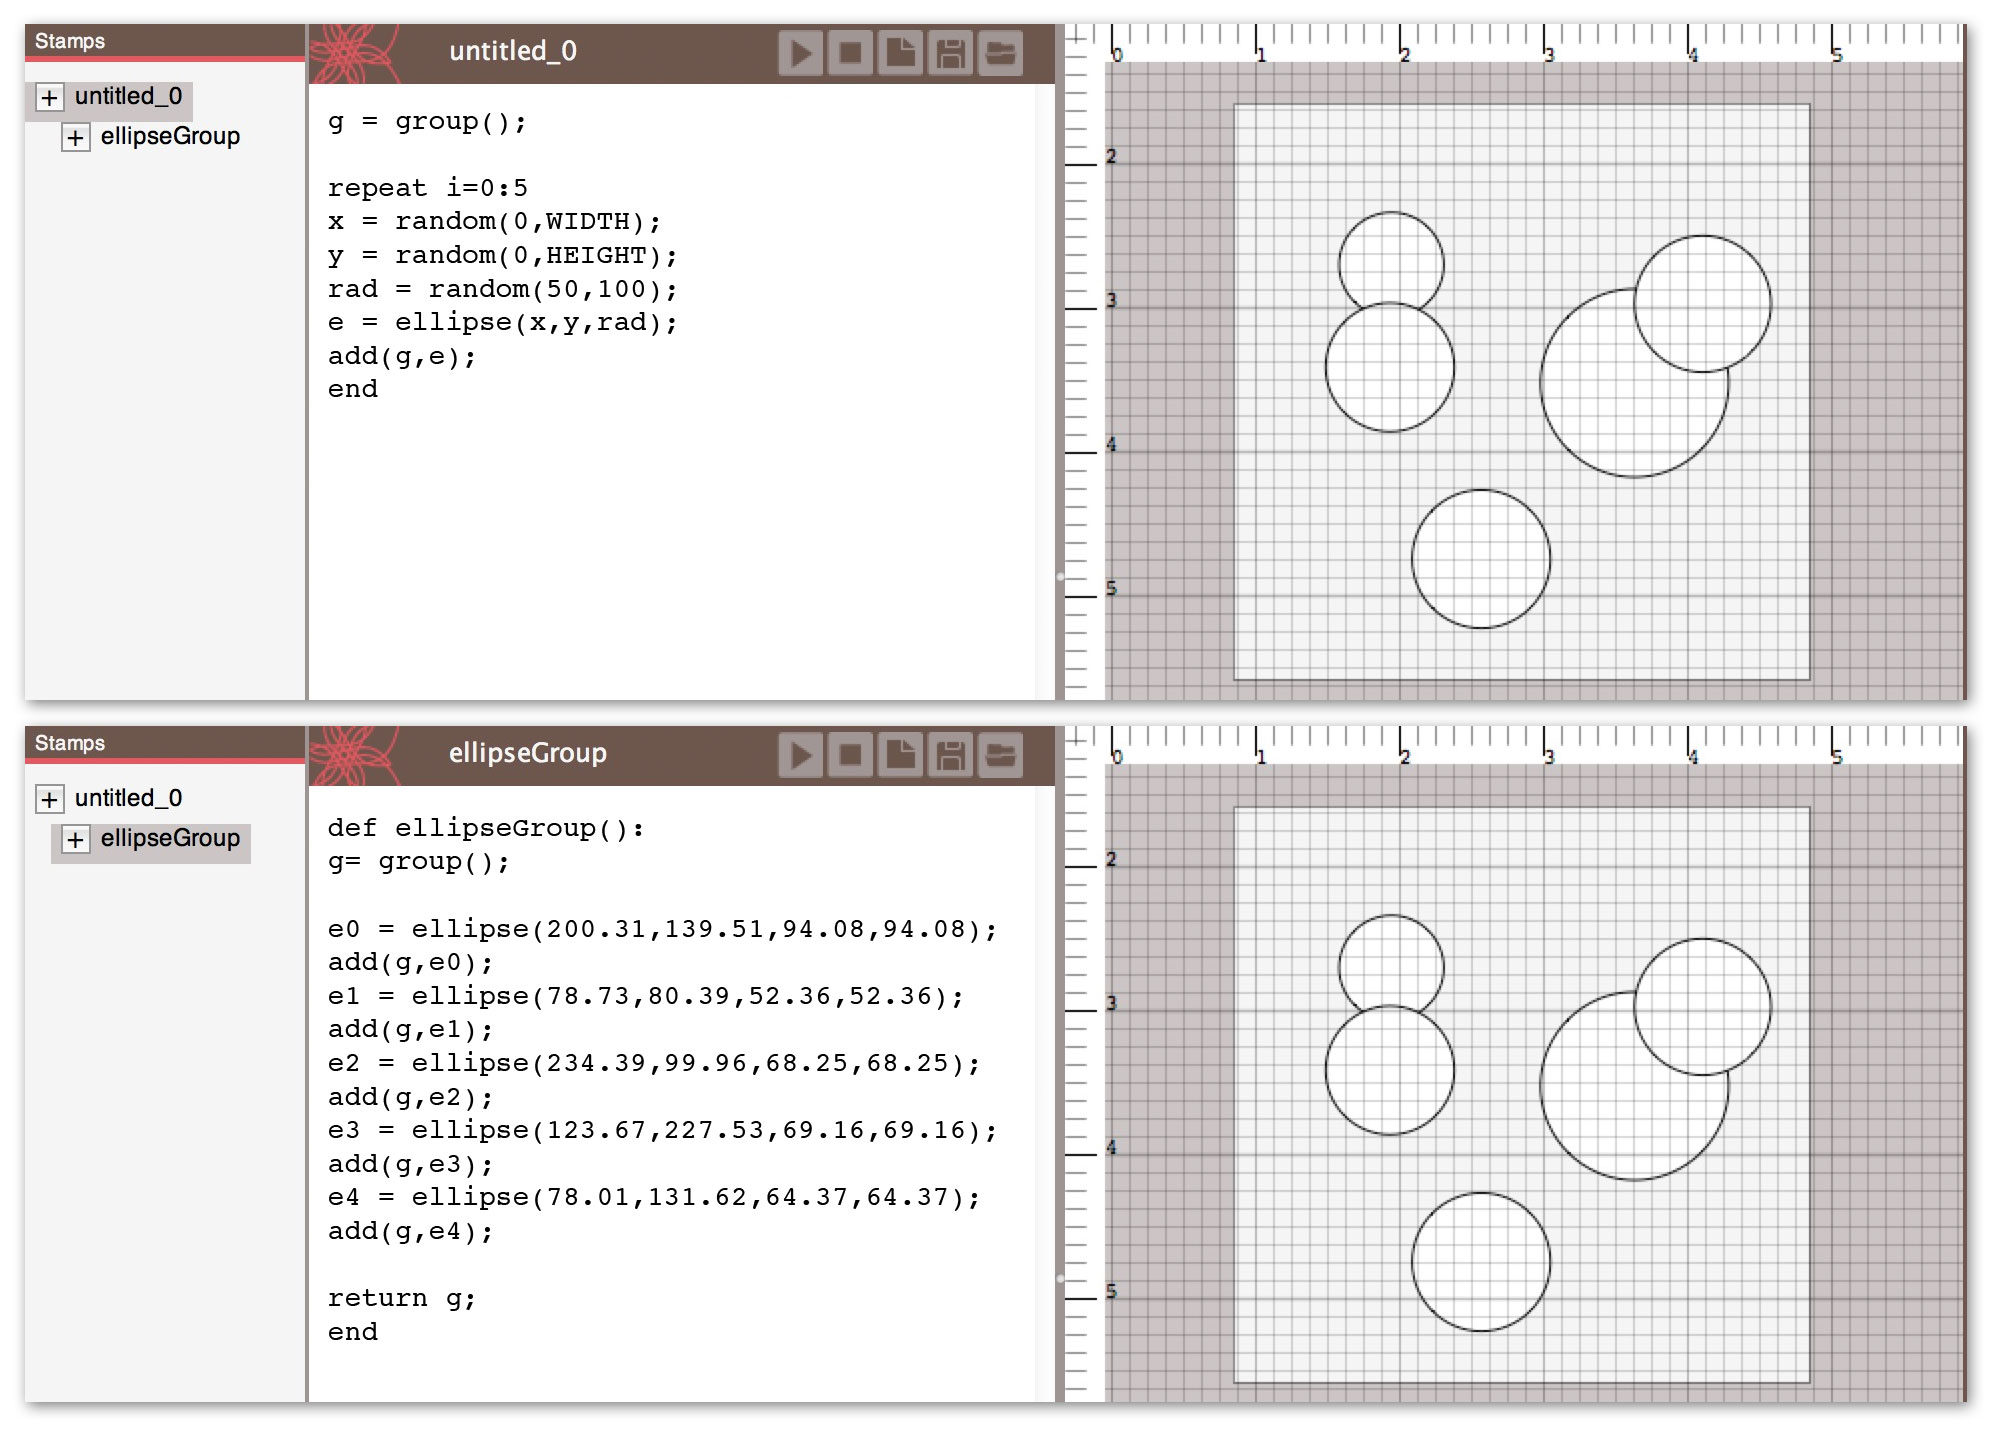
\includegraphics[width=\columnwidth]{images/stamps.jpg}
\caption{Static stamp functionality. (Top: design defined code which generates five random ellipses. The ellipses' positioning and size will change each time the program is run. Bottom: static stamp created from ellipses which will always return the same design.)}
\label{fig:stamps}
\end{figure}
\end{center}
\vspace{-20pt}
\section{Development Process}
\subsection{Initial Development Objectives}
\subsection{First Workshop}
\subsection{Second Workshop}
\section{Discussion}
\section{Conclusion}
\balance

% REFERENCES FORMAT
% References must be the same font size as other body text.

\bibliographystyle{acm-sigchi}
\bibliography{dresscode}
\end{document}